%%%%%%%%%%%%%%%%%%%%%%%%%%%%%%%%%%%%%%%%%%%%%%%%%%%%%%%%%%%
% --------------------------------------------------------
% RMxAA Rho
% LaTeX Template
% Version X.X.X (25/06/2025)
%
% Authors: 
% Carlos Román-Zúñiga (croman@astro.unam.mx)
% Irene Cruz-Gonzaélz )icruzgonzalez@astro.unam.mx)
% Contributors:
% Guillermo Jimenez (memo.notess1@gmail.com)
% Eduardo Gracidas (eduardo.gracidas29@gmail.com)
% 
% License:
% XXXXXXXXXX
% --------------------------------------------------------
%%%%%%%%%%%%%%%%%%%%%%%%%%%%%%%%%%%%%%%%%%%%%%%%%%%%%%%%%%%
% --------------------------------------------------------
%                     ACKNOWLEDGMENTS
% This template has been developed based on the original rho 
% LaTeX class work, created by Luis Guillermo Jimenez Lopez 
% and Eduardo Gracidas Reyes. Available in the Overleaf's 
% template gallery.
% --------------------------------------------------------
%%%%%%%%%%%%%%%%%%%%%%%%%%%%%%%%%%%%%%%%%%%%%%%%%%%%%%%%%%%

% Sugerencia de usar 9pt 
\documentclass[9pt,article,twoside]{rmaa-rho-class/rmaa-rho}
\RMxAAtemplatetype{\RMxAA} % Select your article type
% {\RMxAA} article template
% {\RMxAC} conference template

\newcommand\rmaatex{RMxAA~\LaTeX}
\newcommand{\CS}[1]{\texttt{\textbackslash #1}}

%----------------------------------------------------------
% JOURNAL/HEADER INFORMATION
%----------------------------------------------------------

\vol{61}
% Counter page
\setcounter{page}{30}
\pages{30-36}
\thisyear{2025}
\doi{\href{https://www.astroscu.unam.mx/rmaa/RMxAA..XX-X}{https://www.astroscu.unam.mx/rmaa/RMxAA..XX-X}}

\newenvironment{Example}
{\begin{list}{}{\setlength{\leftmargin}{10pt}\setlength{\rightmargin}{10pt}}%
  \item[]\itshape}
  {\end{list}}

%----------------------------------------------------------
% TITLE
%----------------------------------------------------------

\title{\rmaatex ~ template for article preparation  v4.1}

%----------------------------------------------------------
% AUTHORS AND AFFILIATIONS
%----------------------------------------------------------

\author[1,$\dagger$]{C.~G.~ Román-Zúñiga \orcidlink{0000-0001-8600-4798}}
\author[2,$\dagger$]{I.~Cruz-González \orcidlink{0000-0002-2653-1120}}
\author[3]{W.~J.~Henney \orcidlink{0000-0001-6208-9109}}
\author[1,2,$\dagger$]{A. Student}
\author[2,4]{M.~Y.~Posdoc}

%----------------------------------------------------------

\affil[1]{Universidad Nacional Autónoma de México, Instituto de Astronomía, AP 106,  Ensenada 22800, BC, México}
\affil[2]{Universidad Nacional Autónoma de México, Instituto de Astronomía, AP 70-264, CDMX 04510, México}
\affil[3]{Universidad Nacional Autónoma de México, Instituto de Radioastronomía y Astrofísica. Antigua Carretera a Pátzcuaro 8701, Ex-Hda. San José de la Huerta, 58089, Morelia, Michoacán, México}
\affil[4]{One more affiliation you may need}
\affil[$\dagger$]{This project is part of a collaboration/consortium/program}
%----------------------------------------------------------
% CORRESPONDING AUTHOR INFORMATION
%----------------------------------------------------------

\leadauthor{Román-Zúñiga et al.}
\smalltitle{LaTex Macro RMxAA}

%----------------------------------------------------------
% ARTICLE INFORMATION
%----------------------------------------------------------

\corres{Carlos Román-Zúñiga}
\email{croman@astro.unam.mx}

\received{April 16th, 2024}
%\revised{April 16, 2024}
\accepted{\today}
%\published{May 21, 2024}

\license{Texto de la licencia aquí}

% incluir Resumen y Abstract

\setbool{rho-abstract}{true} % Set false to hide the abstract
\setbool{rho-resumen}{true} % Set false to hide the abstract

%----------------------------------------------------------
% ABSTRACT AND kEYWORDS
%----------------------------------------------------------

\begin{abstract}
    This document (\texttt{rmxaa$\_$main.tex}---last updated August 2025) provides a brief tutorial on the use of version 4.1 of the \texttt{\rmaatex} macros and can also serve as  a template for the preparation of papers to be published in the Main Journal of the Revista Mexicana de Astronomía y Astrofísica. It provides brief tutorial information and common rules for authors. We have included information about the section content, as well as examples of the figures, tables, and code lines. We are making use of the rho($\rho$) \LaTeX ~class, specially designed for academic purposes. It is assumed that you are already familiar with the rudiments of \LaTeX{}. In case you are not, we recommend the manuals provided by Overleaf (\url{https://www.overleaf.com/learn/latex/Tutorials}).
\end{abstract}

\keywords{keyword 1, keyword 2, keyword 3, keyword 4, keyword 5}

%----------------------------------------------------------
% RESUMEN Y PALABRAS CLAVES
%----------------------------------------------------------

\begin{resumen}
    Este documento (\texttt{rmxaa$\_$main.tex}--- última actualización Agosto, 2025) describe de manera breve el uso de la versión 4.1 de los macros \texttt{\rmaatex} y funciona como un templete común para la preparación de artículos que se deseen publicar en la parte principal de la Revista Mexicana de Astronomía y Astrofísica. El documento provee textos instructivos breves y reglas básicas para los autores. hemos incluído información sobre el contenido de las secciones, así como ejemplos de figuras, tablas y la inclusión de líneas de código. Se hace uso de la clase rho ($\rho$) \LaTeX, especialmente diseñada para propósitos académicos. Se asume que el autor está familiarizado con los rudimentos de \LaTeX{}. En caso de que no sea así, recomendamos los manuales que provee la plataforma Overleaf (\url{https://www.overleaf.com/learn/latex/Tutorials}).
\end{resumen}


%\pclave{palabra clave 1, palabra clave 2, palabra clave 3}

%----------------------------------------------------------

\begin{document}

\maketitle
\pagestyle{fancy}\thispagestyle{firststyle}

%----------------------------------------------------------

\section{INTRODUCTION}

    \RMxAAstart{W}elcome to the \rmaatex template to prepare your academic article. Articles considered for publication in the main journal can be easily prepared using this template. The style of this template is based on the \textit{rho class} style\footnote{The RMxAA paper template is based on the rho LATEX class,
created by Luis Guillermo Jiménez López and Eduardo Gracidas Reyes.}. It requires minimal or no typesetting adjustments to provide a version of your manuscript organization that is close to the final printed version. This style also has ample margins to allow for a comfortable number of words per line and leaves room for marginal notes to be added.

    The version of the rmaa-rho document class described in this User Guide is 1.0 (\today). Its use requires a relatively recent version of \LaTeX{}, although it is optimized to work directly online using \textbf{Overleaf}. The current version of the \LaTeX{} Project Public License is 1.3c (2008).  For the author who requires a general introduction to \LaTeX{}, we recommend starting at The LaTeX Project website \url{https://www.latex-project.org/about/}, or using the Overleaf LaTeX guide \url{https://www.overleaf.com/learn/latex/Free_online_introduction_to_LaTeX_(part_1)}. 

\section{PREAMBLE}

    The first line to appear in your document should be 

    \bigskip
    \CS{documentclass}\verb+{rmaa-rho}+
    
    \bigskip
    or
    
    \bigskip
    \CS{documentclass}[\textbf{optionlist}]\verb+{rmaa-rho}+
    
    \bigskip
    \noindent which configures the document to use the rmaa class, using the default \texttt{manuscript} option, which is designed for use by authors who submit articles to the main RMxAA journal. The following commands can be used after the \verb|documentclass| command, but before \verb|\begin{document}|.

    \subsection{Title}

        The \CS{title} command defines the article title. The title text should be entered in mixed case letters. In general, for archival and reference purposes, it is recommended not to use mathematical expressions in a title, but they are allowed if necessary. 

        \bigskip
        \verb|\documentclass{title text}|
        \bigskip

    \subsection{Author information}
    
        The \CS{author} command defines the article’s authors. In addition to this command, the \CS{affil} command can be used to define authors’ affiliations. This will be typed below the authors’ names in the final version of the manuscript. Individual authors should be entered in the style \texttt{A.\~{}B.\~{}Lastname} to avoid line breaks within the name. Authors may use their first name instead of the initial before their second initial and last name.  Line breaks may be inserted by hand using a double backslash symbol “\CS \CS". If the authors have various affiliations, you can put more than one of them in square brackets preceding the author name, as in the example below: Note that we also included the ORCID number and link for each author.
    
        \bigskip
        
        \CS{author}[{affiliation list}]\verb|{author first & last name}|  \CS{orcidlink} \verb|{author ORCID}|
        
        \bigskip
        and the affiliation details with the command line
        
        \bigskip
        \CS{affil}[\textbf{number or symbol}]\verb|{affiliation text}|

        \bigskip
    
    \subsection{Footer information}
    
        The \CS{leadauthor} command is used to provide the last name and initials of the leading author of the article, and will be visible at the top of every odd-numbered page. Please do not modify the text of the \CS{smalltitle} and \CS{institution} commands, which define the footer text at the bottom of the first page of every article in the RMxAA.
    
    \subsection{Corresponding author information}
    
        Please use the \CS{corres} and \CS{email} commands to define the name and e-mail address of the corresponding author. In most cases, this will probably coincide with the lead author, as in the example. We note that the only email used in the manuscript is that of the corresponding author; the remaining authors are identified by their ORCID and affiliations.

        \subsection{Keywords}

        Keywords are provided by the authors and placed below the author´s addresses. A minimum of three keywords and a maximum of five keywords must be placed using the command \verb|\keywords{}|.
    
    \subsection{Abstract}
    
        In this section, you need to provide the abstract in both Spanish and English. The abstract text may contain several paragraphs, but it should not be overly long, since both abstracts must fit on the first page\footnote{this is a footnote}. The recommended length is 200 words for both English and Spanish abstracts. If the authors are unable to provide a Spanish version of the abstract, you can use the same text as the English abstract, and our editors will take care of it.
    
        The text for the {\bf abstract} and the {\bf resumen} is placed with the \verb|\begin{abstract} \end{abstract}| and \verb|\begin{resumen} \end{resumen}| commands, respectively. 
        
        %Below the abstract, a minimum of three keywords and a maximum of five keywords must be placed using the command \verb|\keywords{}|. %Equivalently, the keywords provided as "palabras clave" in Spanish using the command \verb|\pclave{}| will be taken care of by the editors.

        \begin{figure}[ht]
            \centering
            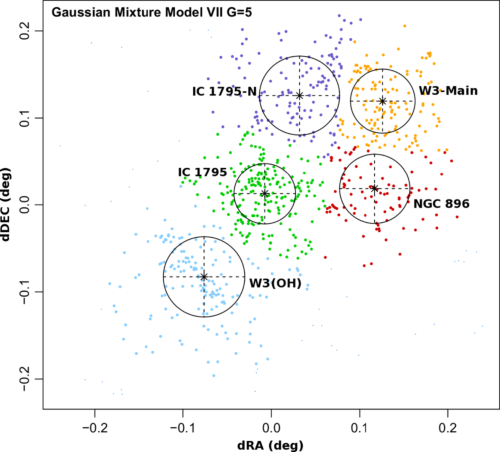
\includegraphics[width=0.99\columnwidth]{figures/GMM_W3.pdf}
            \caption{Example figure, from \cite{Roman+15}.}
            \label{fig:figure1}
        \end{figure}

\section{MAIN BODY}

    The main body of the document should be opened within the following pair of commands:
    
    \bigskip
    \CS{begin}\verb+{document}+
    
    ...
    
    ARTICLE TEXT
    
    ...
    
    \CS{end}\verb+{document}+
    \bigskip
    
    The first command after the \CS{begin}\verb+{document}+ should be \CS{maketitle}. This will format the Title, Author(s), Abstract, Resumen, and Keywords sections.
    
    Within the main body of the document, all standard \LaTeX{} commands can be used. The commands provided by many optional packages distributed with \LaTeX{} may also be used as long as the package is loaded using the \CS{usepackage} command in the preamble. However, authors are requested to avoid using commands that change the document fonts, page layout, or other 'stylistic' parameters. We should also note that not all optional packages have been tested for compatibility with the rmaa\_rho class.

    \begin{figure*}[t]
        \centering                
        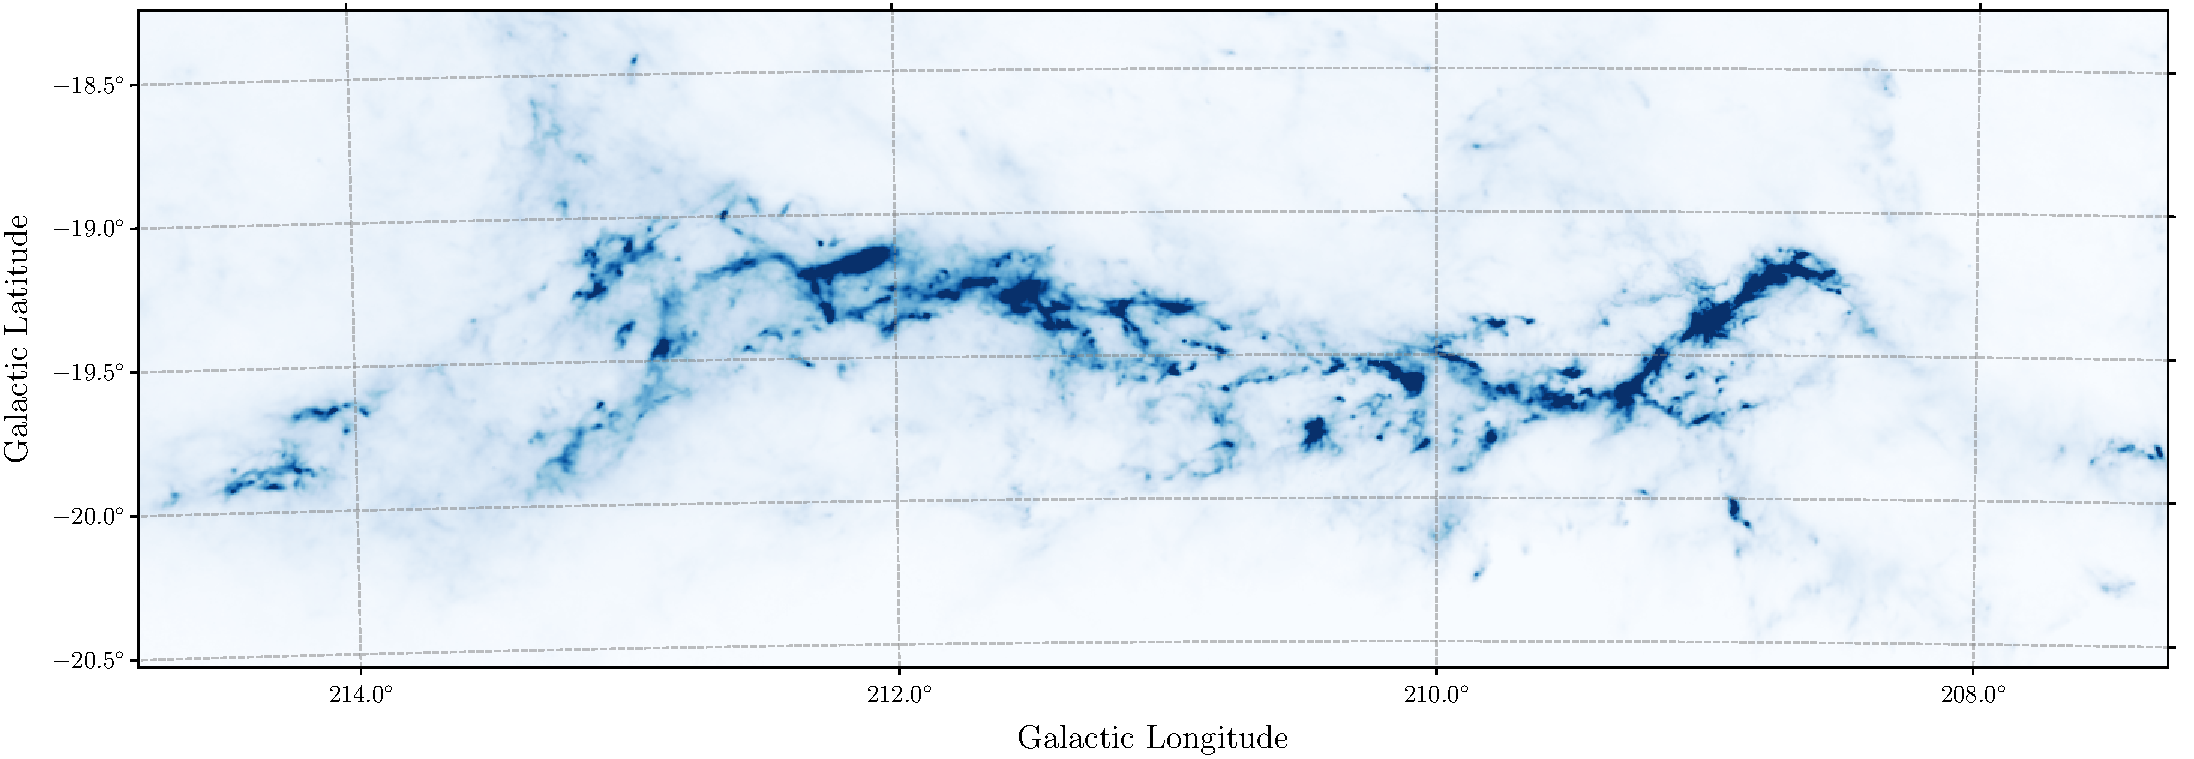
\includegraphics[width=\textwidth]{figures/OrionAvMap.pdf}
        \caption{Second example figure}
        \label{fig:figure2}
    \end{figure*}

\subsection{Sectioning commands and cross references}

    Authors are encouraged to use the standard \LaTeX{} sectioning commands to subdivide their articles as follows:

    \bigskip
    \CS{section}
    
    \CS{subsection}
    
    \CS{subsubsection}
    
    \CS{paragraph}
    \bigskip

    Please use standard \LaTeX\ sectioning commands to subdivide your document. You should use mixed cases for the section titles, although in the current style, this only matters at the level of \CS{subsection} and below.

    These will be automatically typed in the RMxAA style. Cross-referencing is made easier by the use of the \CS{label} \verb+{LABEL}+ command immediately after each sectioning command, where the LABEL text is a mnemonic string. Elsewhere in the document, the section can then be referred to as \S \CS{ref} \verb+{LABEL}+. The \CS{label} command can also be used with equations, figures, and tables (see below). 

    It is preferable to use the \CS{label}/\CS{ref} mechanism for cross-references to minimize the chance of errors and allow automatic hyperlinks in the PDF output. The style that should be used for cross-references is, for example, Figure 3, Table 1, Equation (12), and \S 5.1, where the symbol of the section “§” is produced by the \LaTeX{} command “\S” \ S.

    \subsection{Math Symbols and Equations} \label{sec:math}

        Symbols for physical quantities should usually be in italics: velocity, $v$, density, $N$, etc. However, multi-letter symbols generally look better in Roman: FWHM, EM, etc. 
    
        The subscripts should be in roman (coded using \CS{mathrm}) unless they are themselves variables: $N_\mathrm{e}$, $T_\mathrm{eff}$, but $\sum_i a_i$. 
        
        Physical units should be in roman with thin spaces: $10\,\mathrm{K}$, $1.2\times10^{-12}\,\mathrm{erg\,cm^{-2}\,s^{-1}}$, etc. 
    
        Things generally come out best if you place an entire expression within a single pair of \$'s and then make judicious use of \CS{mathrm}. For example,
    
        \begin{Example}
          $ \mathrm{FWHM} = \int N_\mathrm{e} N_\mathrm{i} \, dz $ 
        \end{Example}
    
        Recall that the ``minus sign'' only exists inside math mode: minus two is $-2$, not~-2, nor \hbox{even --2!} In addition, remember that spacing inside math mode is designed for equations, not words, so you should not use \$'s just to get italic text. Compare $eff$ and \textit{eff}. 
    
        The \CS{frac} command (and its \TeX{} relative \CS{over}) is best used only in displayed equations, as in this case: Something like 
    
        \begin{equation} \label{ec:Equation1}
            x = \frac { a + b } { c } 
        \end{equation}
    looks fine, whereas $x = \frac { a + b } { c }$ looks somewhat cramped. It is better rewritten as $x = (a + b) / c $. 
    
        \paragraph{How to define a macro that can be used inside or outside math mode.} Use the \CS{ensuremath} command. For example: 
    
\begin{verbatim}
\newcommand{\fluxunits}{%
    \ensuremath{\mathrm{%
        erg\,s^{-1}\,cm^{-2}}}}
\end{verbatim}
    
        Then you can write either \verb+15.1\,\fluxunits+ or \verb+$2.3\times+ \verb+10^{-11} \,+ \verb+\fluxunits$+
    
        \paragraph{How to define a macro that can be used inside or outside math mode.} Use the \CS{ensuremath} command. For example: 
        
\begin{verbatim}
\newcommand{\fluxunits}{%
    \ensuremath{\mathrm{%
        erg\,s^{-1}\,cm^{-2}}}}
\end{verbatim}
    
        Then you can write either \verb+15.1\,\fluxunits+ or \verb+$2.3\times+ \verb+10^{-11} \,+ \verb+\fluxunits$+

    \subsubsection{Equations}

        Equation~\ref{ec:equation2} shows the Schrödinger equation as the first example of an elegant equation with a proper label.

    \begin{equation} \label{ec:equation2}
         \frac{\hbar^2}{2m}\nabla^2\Psi + V(\mathbf{r})\Psi = -i\hbar \frac{\partial\Psi}{\partial t}
    \end{equation} 

    Equation~\ref{ec:equation2} shows the Riemann tensor as a slightly more complicated example using sub- and superscripts.

    \begin{equation} \label{ec:equation3}
        R^\alpha\,_{\epsilon\mu\nu}:=\partial_\mu\Gamma^\alpha\,_{\nu\epsilon}
	-\partial_\nu\Gamma^\alpha\,_{\mu\epsilon}
	+\Gamma^\sigma\,_{\nu\epsilon} \Gamma^\alpha\,_{\mu\sigma}
	-\Gamma^\sigma\,_{\mu\epsilon} \Gamma^\alpha\,_{\nu\sigma},
    \end{equation}
    which, after contraction of the first and third indices, $R_{\mu\nu}:=R^\alpha\,_{\mu\alpha\nu}$, yields an expression (\ref{ec:equation4}) that helps exemplify the use of \textit{splitting} \citep{BarMen17}:

    \begin{equation} \label{ec:equation4}
	\begin{split}
    	R_{\mu\nu}&=R_{\mu\nu}(\{\})
    	+\tilde{\nabla}_\nu K^\alpha\,_{\alpha\mu}
    	-\tilde{\nabla}_\alpha K^\alpha\,_{\nu\mu}\\
    	&+K^\sigma\,_{\nu\mu} K^\alpha\,_{\alpha\sigma}
    	-K^\sigma\,_{\alpha\mu} K^\alpha\,_{\nu\sigma},
	\end{split}
    \end{equation}

    In another complex expression by the same authors, we can show the addition of intercalated text (italics) in the combined Eqs. ~\ref{ec:equation5} and ~\ref{ec:equation6}

    \begin{gather}
	\begin{split}
		&R_{\mu\nu}\{\}-\frac{1}{2}g_{\mu\nu}R\{\}
			-\frac{1}{2}g_{\mu\nu}\kappa(\tilde{\nabla}_\alpha
			T^\alpha+ T^\alpha T_\alpha)^b\\
		&+\kappa b(\tilde{\nabla}_\alpha T^\alpha+T^\alpha
			T_\alpha)^{b-1}T_\mu T_\nu \\ 
	        & -\kappa bT_\nu \tilde{\nabla}_\mu\left[(\tilde{\nabla}_\alpha
			T^\alpha+ T^\alpha T_\alpha)^{b-1}\right]\\
		&=\frac{8\pi G}{c^4} \Sigma_{\mu\nu},
	\end{split}
	\label{ec:equation5}
	\\
	\intertext{\textit{for the null variations with respect to the metric, and}}
	2T_\mu(\tilde{\nabla}_\alpha T^\alpha+ T^\alpha T_\alpha)^{b-1}=
		\tilde{\nabla}_\mu\left[(\tilde{\nabla}_\alpha T^\alpha+ T^\alpha T_\alpha)^{b-1}\right]
	\label{ec:equation6}
    \end{gather}

    \subsection{Special symbols}

        The commands for the commonly used symbols in astronomy are listed in Table~\ref{tab:anysymbols}.

        \begin{table}[ht]
            \caption{Astronomy special symbols commands.} 
            % Additional commands for special symbols commonly used in astronomy. These can be used anywhere.}
            \label{tab:anysymbols}
            \centering
            \begin{tabular*}{0.9\columnwidth}{@{}l@{\hspace*{20pt}}l@{\hspace*{20pt}}l@{}}
                \toprule
                Command & Output & Meaning\\
                \midrule
                \verb'\sun' & \sun & Sun, solar\\[2pt] % additional height spacing for enhanced symbol legibility
                \verb'\earth' & \earth & Earth, terrestrial\\[2pt]
                \verb'\micron' & \micron & microns\\[2pt]
                \verb'\degr' & \degr & degrees\\[2pt]
                \verb'\arcmin' & \arcmin & arcminutes\\[2pt]
                \verb'\arcsec' & \arcsec & arcseconds\\[2pt]
                \verb'\fdg' & \fdg & fraction of a degree\\[2pt]
                \verb'\farcm' & \farcm & fraction of an arcminute\\[2pt]
                \verb'\farcs' & \farcs & fraction of an arcsecond\\[2pt]
                \verb'\fd' & \fd & fraction of a day\\[2pt]
                \verb'\fh' & \fh & fraction of an hour\\[2pt]
                \verb'\fm' & \fm & fraction of a minute\\[2pt]
                \verb'\fs' & \fs & fraction of a second\\[2pt]
                \verb'\fp' & \fp & fraction of a period\\[2pt]
                % \verb'\diameter' & \diameter & diameter\\[2pt]
                \verb'\sq' & \sq & square, Q.E.D.\\[2pt]
                \bottomrule
            \end{tabular*}
        \end{table}

    \subsection{Ionization states}




        For ions, a \verb'\ion{}{}' command is used for the correct typesetting of ionization states. For example, to typeset singly ionized calcium, use \verb'\ion{Ca}{ii}', which produces \ion{Ca}{ii}, while a double-ionized oxygen forbidden line produces [\ion{O}{iii}].


    \section{CONCEPT HIGHLIGHT BOX} 

    The new \rmaatex\ macro allows the authors to use a colored box to highlight a concept or equation, as shown in this example. The label and reference points of the section are included. Example: See the Concept box in Section~\ref{box:box1}.  


    \begin{figure*}[ht]
        \centering
        \begin{subfigure}[b]{0.38\linewidth} % Fig (a)
            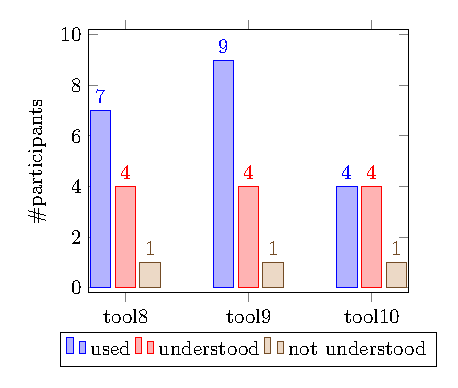
\includegraphics[width=\linewidth]{figures/bar-plot.pdf}
            \caption{Example left figure.}
            \label{fig:figa}
        \end{subfigure}
        \hspace{15pt}   % Space between the figures
        \begin{subfigure}[b]{0.38\linewidth} % Fig (b)
            \centering
            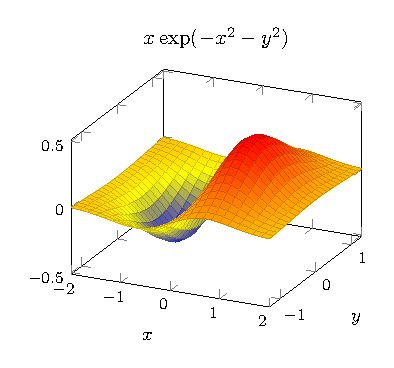
\includegraphics[width=\linewidth]{figures/surface-plot-math.pdf}
            \caption{Example right figure.}
            \label{fig:figb}
        \end{subfigure}
        \caption{\justifying Example figure that covers the width of the page obtained from PGFPlots \cite{PFGPlots}. In this case, the caption length is quite long, so it is justified at the edges.}
        \label{fig:examplefloat}
    \end{figure*}


    
    \begin{rhoenv}[frametitle=Highlight Concept Box]
        Hello! This is an example of a concept highlight box (HCB) section. I can be placed anywhere in the body of the paper to briefly summarize the important concepts. We do not allow HCBs larger than 40 words \label{box:box1}
    \end{rhoenv}

\section{FIGURES AND TABLES}

       \begin{table*}[hb]
            \RaggedRight
            \caption{Table example that covers the width of the page.}
            \label{tab:pwtable}
                \begin{tabular}{lllp{10cm}}
                    \toprule
                    \textbf{Day} & \textbf{Min Temp} & \textbf{Max Temp} & \textbf{Summary} \\ 
                    \midrule
                    Monday & 11\textdegree C & 22\textdegree C & A clear day with lots of sunshine.  Strong breezes lower temperatures. \\
                    Tuesday & 9\textdegree C & 19\textdegree C & Cloudy with rain across many northern regions. \\
                    Wednesday & 10\textdegree C & 21\textdegree C & Rain will still linger for the morning. 
                    Conditions will improve by early afternoon and continue 
                    throughout the evening.\\
                    \bottomrule
                \end{tabular}    
            \tabletext{Note: Obtained from Latex tables \cite{projects-2023}.}
        \end{table*}

    \subsection{Sample simple figure}

        Figure~\ref{fig:figure1} shows an example of a simple figure occupying the space of a single column. In most cases, this is a good option for displaying a relatively simple scatter plot or histogram. We require that the font of the axis labels be at least as large as that of the caption.
        
     \subsection{Sample wide figure}

        Figure~\ref{fig:figure2} shows an example of another relatively simple figure, but this time the width of the figure is as large as the width of the page. In this example, the figure is placed at the top of the page.

            
    \subsection{Sample double figure}

        Figure~\ref{fig:examplefloat} shows an example of a floating figure with two separate panels covering the width of the page. The figure can be placed at the top or bottom of the page. The space between the figures can also be modified using the \verb|\hspace{Xpt}| command.


    \subsection{Sample simple table}

        Similar to figures, tables can be placed in one or two columns, depending on their length.

        Table~\ref{tab:anysymbols} is an example of a relatively simple table, with three columns, which is narrow enough to be shown inside a single column. The example is also useful as a quick guide to the symbols commonly used in astronomy.

\subsection{Sample wide table}

        Table~\ref{tab:pwtable}, shows a second example of a table. This time, the content of the table is more adequate for a larger horizontal size. The example is constructed such that the table covers the width of the page and is positioned at the bottom of a new page.

\subsection{Landscape table}
    
 The third example of tables is shown in Table~\ref{tab:pwlstable}, where we show a more complex table rotated sideways to fit in the landscape mode. 

 RMxAA uses the \LaTeX package \texttt{tabular}, which is adequate for most applications in this context. A good tutorial for tables, with direct applications of the \texttt{tabular} can be found in \url{https://www.overleaf.com/learn/latex/Tables}. 

 We do not recommend publishing very long tables in your paper. Large data collections may be more useful to readers in a machine-readable format (MRT). In the manuscript, a table with fewer rows may serve as a guide for the content of the MRT document. Please contact our editors to allocate direct link access to MRT tables in the RMxAA web page for the published version of your manuscript. 

%\newpage

\section{FACILITIES}

For observational research, authors must include a brief list of facilities and instruments used, as well as proper acknowledgment of public catalogs and virtual observatory resources.

\section{REFERENCE STYLE}

    Our default formatting for references uses the journal-naming system from the AASTex style and the Astrophysics Data System (ADS). RMxAA follows the ADS bibliographic codes for both refereed \url{https://adsabs.harvard.edu/abs_doc/refereed.html} and non-refereed \url{https://adsabs.harvard.edu/abs_doc/non_refereed.html} publications.
    
    If a paper has more than five authors, only the first three will be listed, followed by ``et al.". The DOI of each publication was also included in the dataset. At the end of this document, you will find an example of the default reference formatting. 

    The default formatting for references follows the Astrophysics Data System (ADS) BibTeX style. The author should provide a bibliography file using the command \CS{bibliography}\verb|{bibfile}|, where all references are included. At the end of this document, you will find an example of the default reference formatting. Note that the DOI code is linked to references that have one; therefore, it is important to include it in the BibTeX bibliography \texttt{(.bib)} file.
    
    The usual commands \CS{citep} for reference in parentheses, as in \citep{Roman23},  and \CS{citet} for references with year in parentheses, as in \citet{Roman23}, are used in the main body of the article.

    Authors must include their bibliography file with their manuscript, i.e. the 
    bib file. The {\bf rmxaa.bib file} is an example of a bib file that serves as a guide.
%----------------------------------------------------------

\renewcommand{\refname}{REFERENCES}
\bibliography{rmaa}

%----------------------------------------------------------

%\onecolumn
\begin{landscape}
\begin{table*}[htbp]
  \centering\small
  \caption{My Results \label{tab:pwlstable}}
    \begin{tabular}{rrrrrrrrrrrr}
    \toprule
    \textbf{FF} & \textbf{} & \textbf{} & \textbf{AA} & \textbf{BB} & \textbf{CC} & \textbf{DD} & \textbf{FF} & \textbf{GG} & \textbf{HH} & \textbf{II} & \textbf{JJJJ} \\
    \midrule
    \textbf{Ccccccccccc} & \multirow{2}[2]{*}{\textbf{aaaaa aaaaa}} & \multirow{2}[2]{*}{\textbf{aa aa aaaaaa}} & \multirow{2}[2]{*}{\textbf{aaa}} & \textbf{aaaa} & \textbf{aa +} & \textbf{aa +} & \multirow{2}[2]{*}{\textbf{aaa}} & \multirow{2}[2]{*}{\textbf{aaaa aaaaa}} & \textbf{aa +} & \textbf{aa +} & \multirow{2}[2]{*}{\textbf{aaa}} \\
    \textbf{aaaaaaaaaa} &       &       &       & \textbf{aaaaa} & \textbf{a-aaaaa} & \textbf{a-aaaaa} &       &       & \textbf{a-aaaaa} & \textbf{a-aaaaa} &  \\
    \midrule
    \textbf{aaaaaaaa} & \textbf{0000} & \textbf{1111} & 22222 & 333333 & 444444 & 5555  & 66666 & 77777 & 88888 & 99999 & 10100 \\
          & 000   & \textbf{1111} & 22222 & 33333 & 44444 & 55555  & 66666 & 77777 & 88888 & 99999 & 10.10 \\
          & 000   & \textbf{1111} & 22222 & 33333 & 44444 & 55555  & 66666 & 77777 & 88888 & 99999 & 10.10 \\
          & 000   & \textbf{1111} & 22222 & 33333 & 44444 & 55555  & 66666 & 77777 & 88888 & 99999 & 10.10 \\
          & 000   & \textbf{1111} & 22222 & 33333 & 44444 & 55555  & 66666 & 77777 & 88888 & 99999 & 10.10 \\
          & 000   & \textbf{1111} & 22222 & 33333 & 44444 & 55555  & 66666 & 77777 & 88888 & 99999 & 10.10 \\
          & 000   & \textbf{1111} & 22222 & 33333 & 44444 & 55555  & 66666 & 77777 & 88888 & 99999 & 10.10 \\
          & 000   & \textbf{1111} & 22222 & 33333 & 44444 & 55555  & 66666 & 77777 & 88888 & 99999 & 10.10 \\\\
    \textbf{aaaaaaaa} & \textbf{0000} & \textbf{1111} & 22222 & 333333 & 444444 & 5555  & 66666 & 77777 & 88888 & 99999 & 10100 \\
          & 000   & \textbf{1111} & 22222 & 33333 & 44444 & 55555  & 66666 & 77777 & 88888 & 99999 & 10.10 \\
          & 000   & \textbf{1111} & 22222 & 33333 & 44444 & 55555  & 66666 & 77777 & 88888 & 99999 & 10.10 \\
          & 000   & \textbf{1111} & 22222 & 33333 & 44444 & 55555  & 66666 & 77777 & 88888 & 99999 & 10.10 \\
    \textbf{aaaaaaaa} & \textbf{0000} & \textbf{1111} & 22222 & 333333 & 444444 & 5555  & 66666 & 77777 & 88888 & 99999 & 10100 \\
          & 000   & \textbf{1111} & 22222 & 33333 & 44444 & 55555  & 66666 & 77777 & 88888 & 99999 & 10.10 \\
          & 000   & \textbf{1111} & 22222 & 33333 & 44444 & 55555  & 66666 & 77777 & 88888 & 99999 & 10.10 \\
          & 000   & \textbf{1111} & 22222 & 33333 & 44444 & 55555  & 66666 & 77777 & 88888 & 99999 & 10.10 \\
    \textbf{aaaaaaaa} & \textbf{0000} & \textbf{1111} & 22222 & 333333 & 444444 & 5555  & 66666 & 77777 & 88888 & 99999 & 10100 \\
          & 000   & \textbf{1111} & 22222 & 33333 & 44444 & 55555  & 66666 & 77777 & 88888 & 99999 & 10.10 \\
          & 000   & \textbf{1111} & 22222 & 33333 & 44444 & 55555  & 66666 & 77777 & 88888 & 99999 & 10.10 \\
          & 000   & \textbf{1111} & 22222 & 33333 & 44444 & 55555  & 66666 & 77777 & 88888 & 99999 & 10.10 \\
    \midrule
    Aaaaaaa &    & \textbf{0000} & \textbf{11} & \multicolumn{1}{c}{\textbf{22}} & \multicolumn{1}{c}{\textbf{33}} & \multicolumn{1}{c}{\textbf{44}} & \multicolumn{1}{c}{\textbf{55}} & \multicolumn{1}{c}{\textbf{66}} & \multicolumn{1}{c}{\textbf{77}} & \multicolumn{1}{c}{\textbf{88}} & \multicolumn{1}{c}{\textbf{99}} \\
    \bottomrule
    \end{tabular}%
  \label{tab:addlabel}%
\end{table*}
\end{landscape}
%\twocolumn





\section{ACKNOWLEDGEMENTS}

Acknowledgements may be included to recognize funding sources and grants, to provide standardized acknowledgement text (including required references) for facilities or resources, and/or to recognize individuals who contributed to the research with any relevant discussion, resources, or services but are not listed as coauthors.



\section{APPENDICES}

If you have appendices to your article, you can use something like the following:\\
    
    \noindent\CS{begin}\verb|{appendices}|\\
    \CS{section}\verb|{First Appendix}|\\
    \CS{label}\verb|{sec:ap-A}}|\\
    \CS{}\verb|{Text of first appendix.}|\\
    \CS{section}\verb|{Second Appendix}|\\
    \CS{label}\verb|{sec:ap-B}|\\
    \CS{}\verb|{Text of second appendix.}|\\
    \CS{end}\verb|{appendices}|\\

The appendices follow the acknowledgments section but precede the bibliography section. Equations in the appendices are labeled A1, A2, B1, B2, etc..

\section{CODES}

    This macro includes the \textit{listings} package, which offers customized features for adding codes or pseudocodes. The package adds adequate syntax coloring for some of the most popular languages (C, C++, Python, 
    and Matlab).

    \nolinenumbers
    \lstinputlisting[caption=Example of matlab code., 
    label={lst:listing-Mat}, language=Matlab]{examples/codes/example.m}
    \linenumbers

\vspace{2cm}

    \nolinenumbers
    \lstinputlisting[caption=Example of Python code., 
    label={lst:listing-py}, language=Python]{examples/codes/codito.py}
    \linenumbers



    \nolinenumbers
    \lstinputlisting[caption=Example of Pseudo-code., 
    label={lst:listing-pseudo}]{examples/codes/pseudo.p}
    \linenumbers

    During the paper edition process, line numbering will be enabled to facilitate referee revision. We recommend placing the command \verb|\nolinenumbers| at the beginning and \verb|\linenumbers| at the end of the code, respectively. This temporarily removes the line numbering for the manuscript and provides code line numbers.

\end{document}